%-------------- Oliver Pharr   -------------------------------%
\section{Oliver Pharr}
For a definition of the Oliver Pharr method see \cite{OliverPharr}. \\

\begin{figure}[ht]
  \centering
  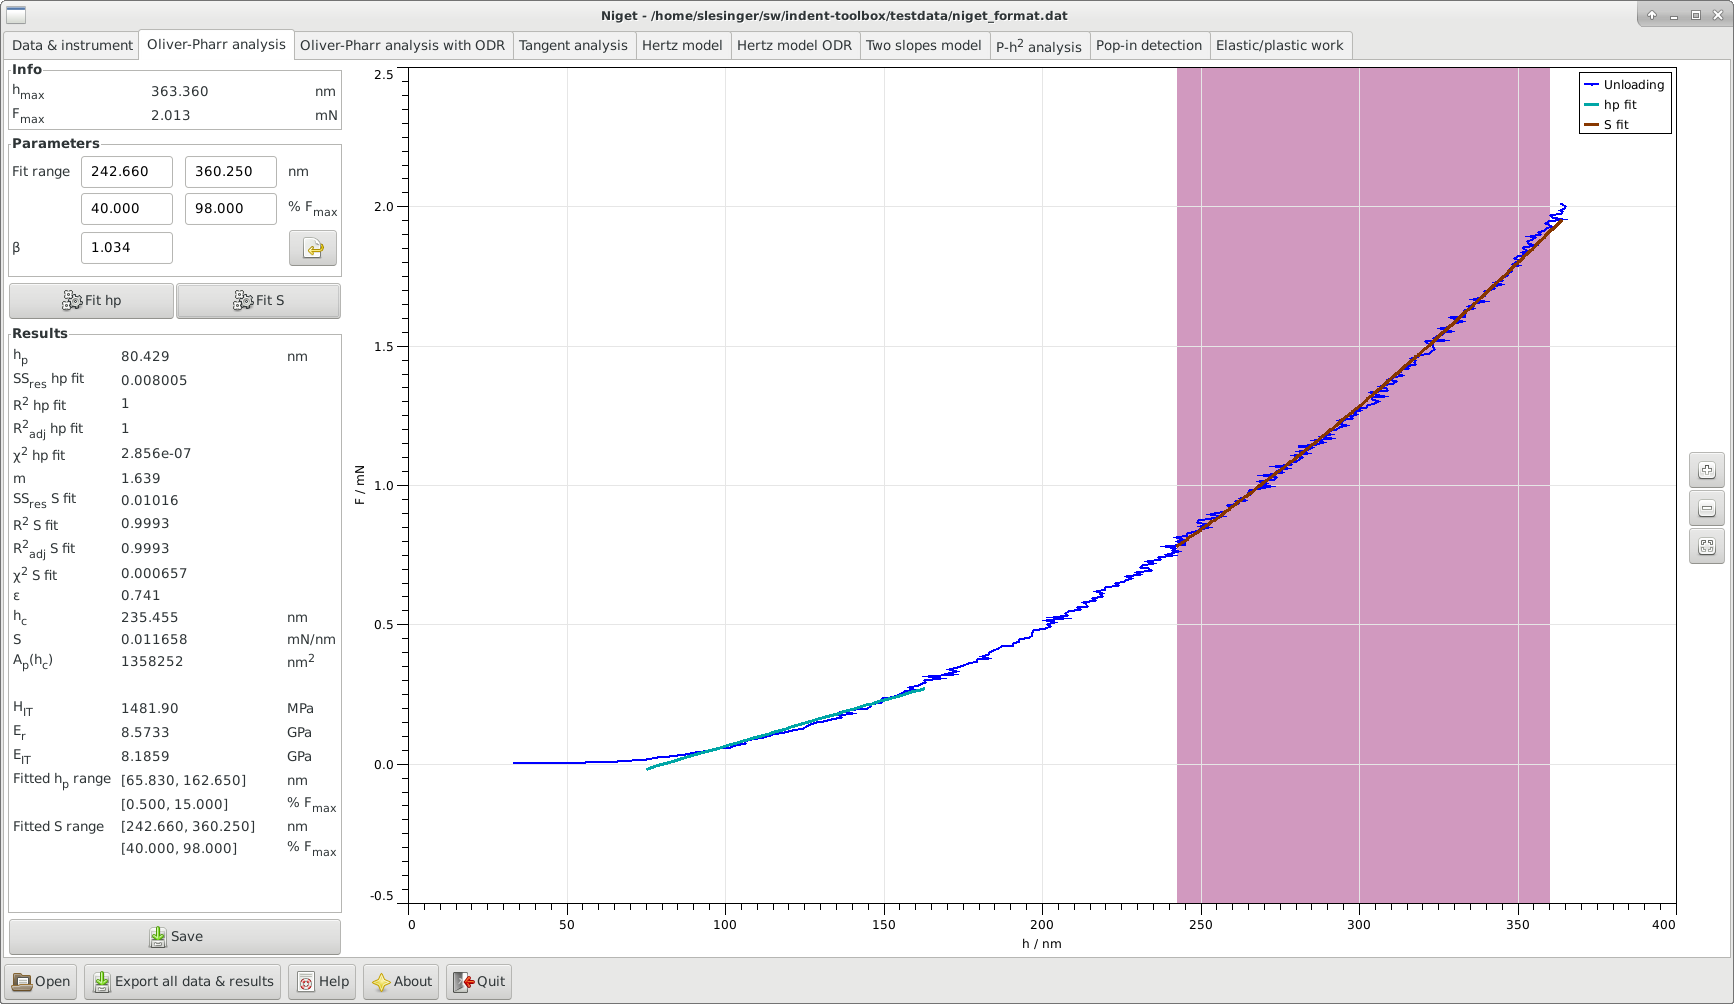
\includegraphics[width=\textwidth]{images/screen-op}
  \caption{Oliver-Pharr analysis}
\end{figure}

\subsection{Window}
The window consists of several blocks:
\begin{itemize}
 \item \emph{Info} displays the maximum depth and force during the indentation
 \item \emph{Parameters} shows the selected range in nm and in \% of the maximum force, and the correction $\beta$. 
        \begin{itemize}
          \item[-] The fitting range can be selected either using the mouse or typing in the range entries. The range can be defined either in nm or in percent of the maximum force. 
                   It is often recommended to use the range 0.5--15~\% F$_\mathrm{max}$ for the hp fit and 40--98~\% F$_\mathrm{max}$ for the S fit, see section \ref{op_calc}.      
          \item[-] The parameter $\beta$ accounts for any deviations from the axisymmetric case and is used in the calculation of the reduced modulus in equation \eqref{eq:Er}. 
                   Currently, the default value is the value for three-sided pyramides $\beta = 1.034$. The value supplied by the user is saved in the settings and can be reset to its default value.
\end{itemize}
\item \emph{Fit} buttons for the two fits, see section \ref{op_calc} for details of the calculation.
\item \emph{Results} displays all results in the following order: the residual depth $\hp$, the power $m$ of the power law function, the parameter $\varepsilon$, 
       the contact depth  $\hc$, the slope $S$, the contact area $\Ap(\hc)$, the indentation hardness $H_{IT}$, the contact modulus $E_r$, the indentation modulus $E_{IT}$ and the ranges used for the fitting procedures.
       The variables are described in detail in section \ref{op_calc}.
 %\item \emph{Uncertainties} show the uncertainty analysis window, see section \ref{op_unc}.
 \item \emph{Save} save parameters and results to given file. 
 \item \emph{Graph} display the unloading curve and the fitted curves.  Stepwise zooming/unzooming can be performed by selecting a range with the mouse and pressing the \emph{Zoom}/ \emph{Unzoom} buttons. The graph is restored to its original size by the \emph{Restore} button.
\end{itemize}

\subsection{Procedure}\label{op_calc}
The standard calculation consists of three steps
\begin{enumerate}
 \item  The residual depth must be determined as the intersection of the unloading curve and the x-axis.
This is implemented by fitting a straight line using a Deming fit with $\delta = 1$, see section \ref{tls}. 
For a brief description of the Deming fit see section \ref{tls}
\begin{equation}
F = \ahp \hp + b_\mathrm{h_{p}} \label{eq:hp-fit}
\end{equation}

using total least squares. This fit is called the $\hp$ fit. The residual depth is calculated as 
\begin{equation} \label{eq:hp}
 \hp = -b_{\hp}/a_{\hp}. 
\end{equation}
The range of the data must be chosen adequately, the range 0.5--15 \% F$_\mathrm{max}$ is often a reasonable value. \\

\item The main part of the unloading curve is fitted by a power law function
\begin{equation}
F = \alpha (h - \hp)^m.
\end{equation}
This is converted to a total least squares fit in the variables using a Deming fit with $\delta =1 $, see section \ref{tls}
\begin{equation}
\log F = \log \alpha + m \log (h- \hp). \label{eq:m-fit}
\end{equation}
The range should not contain the lower part of the unloading range, a range of 40--98~\% F$_\mathrm{max}$ is recommended as a first guess.

\item The auxiliary parameter $\varepsilon$ is calculated from the power $m$
\begin{equation} \label{eq:eps}
\varepsilon = m \left(1-\frac{2(m-1) \Gamma\left(\frac{m}{2(m-1)}\right)}{\sqrt{\pi}\Gamma\left(\frac{1}{2(m-1)}\right)} \right),
\end{equation}
$\Gamma$ is the Gamma-function. \\
The contact depth is calculated as 
\begin{equation} \label{eq:hc}
	\hc=\hmax-\epsilon \frac{\Fmax}{S}
\end{equation}
and the slope at the maximum depth as
\begin{equation} \label{eq:S}
S=m \frac{ \Fmax}{\hmax-\hp}.
\end{equation}
\item 
The contact depth is used to evaluate the contact area $A(\hc)$.
This can be used to find the indentation hardness
\begin{equation}\label{eq:Hit}
\Hit=\frac{\Fmax}{A(\hc)}.
\end{equation}
and together with the slope to find the contact modulus
\begin{equation}\label{eq:Er}
\Er=\sqrt{\pi} \frac{S}{2 \beta \sqrt{A(\hc)}}.
\end{equation}
For a comparison with Young's modulus found in literature it is useful to calculate the indentation modulus $E_{IT}$ 
\begin{equation} \label{eq:Eit}
\Eit = \frac{1 - \nu^2}{1/\Er - (1 - \nui^2) / \Ei}.
\end{equation}
Here $\nu$ is the Poisson's value of the sample and $\nui$ and $\Ei$ are the Poisson's value and the modulus of the indenter. 
\end{enumerate} 
